\documentclass{sig-alternate-05-2015}

%--------------------------------------------------------------------
% Package definitions
\usepackage[utf8]{inputenc}
\usepackage[T1]{fontenc}
\usepackage{lmodern}
\usepackage{balance}
\usepackage{stys/standalone}
\usepackage{stys/relsize}
\usepackage[caption=false, font=footnotesize]{subfig}

\usepackage{url}
\usepackage{ifthen}
\usepackage{cite}
\usepackage{xspace}
\usepackage{pgfplots}
\usepackage{algorithm}
\usepackage{algpseudocode}
\usepackage{epstopdf}
%--------------------------------------------------------------------


%--------------------------------------------------------------------
% Macros
%\newcommand{\comment}[1]{}
\newcommand{\mf}[1]{\mathcal{#1}}
\newcommand{\var}[1]{{\ttfamily#1}}
\newcommand{\Tgran}{\emph{granularity($\mf T$)}\xspace}
\newcommand{\Ggran}{\emph{granularity($\mf G$)}\xspace}
\newcommand{\our}{\mbox{HLens}\xspace}
\newcommand{\tmlda}{\mbox{TM--LDA}\xspace}
\newcommand{\lda}{\mbox{LDA}\xspace}
\newcommand{\atam}{\mbox{ATAM}\xspace}
\newcommand{\tmatam}{\mbox{TM--ATAM}\xspace}
\newcommand{\change}{\emph{\texttt{change-point}}\xspace}
\newcommand{\changes}{\emph{\texttt{change-points}}\xspace}
\newcommand{\season}{\emph{\texttt{homogenous\- time\- period}}\xspace}
\newcommand{\seasons}{\emph{\texttt{homogenous\- time\- periods}}\xspace}
\newcommand{\competitor}{\emph{\texttt{competitor\- topic\- model}}\xspace}
\newcommand{\transition}{\emph{\texttt{transition\- matrix}}\xspace}
\newcommand{\selftransition}{\mbox{stable-topic}\xspace}
\newcommand{\selftransitions}{\mbox{stable-topics}\xspace}
\newcommand{\titleA}{On Harnessing Social Media for Flu Predictions}
\newcommand{\titleB}{How to stop being sick and start enjoying life}
\newcommand{\titleC}{Flu Catcher ! It's like Bird Catcher For Flus}
\newcommand{\titleD}{Health-Lens: Microscopic Ailment Modeling Using Social Media}
\newcommand{\titleE}{Health Monitoring on Social Media over Time}
\renewcommand{\algorithmicrequire}{\textbf{Input:}}
\renewcommand{\algorithmicensure}{\textbf{Output:}}
\DeclareMathOperator*{\argmin}{arg\!min}
\DeclareMathOperator*{\argmax}{arg\!max}
%--------------------------------------------------------------------


%--------------------------------------------------------------------
% Configs
\graphicspath{{./figs/}}
\DeclareGraphicsExtensions{.eps,.jpeg,.png}
%--------------------------------------------------------------------


\begin{document}

\CopyrightYear{2016}
\setcopyright{acmlicensed}
\conferenceinfo{SIGIR '16,}{July      17 - 21, 2016, Pisa, Italy}
\isbn{978-1-4503-4069-4/16/07}\acmPrice{\$15.00}
\doi{http://dx.doi.org/10.1145/2911451.2914697}


\title{\titleE}
\numberofauthors{1} 
\author{
% 1st. author
\alignauthor Sumit Sidana, Shashwat Mishra, Sihem Amer-Yahia,\\ Marianne Clausel, Massih-Reza Amini\\
       \affaddr{Univ. Grenoble Alps/CNRS}\\
       \affaddr{Grenoble, France}\\
       \email{firstname.lastname@imag.fr}
}
% \numberofauthors{5} %  in this sample file, there are a *total*
% % of EIGHT authors. SIX appear on the 'first-page' (for formatting
% % reasons) and the remaining two appear in the \additionalauthors section.
% %
% \author{
% % You can go ahead and credit any number of authors here,
% % e.g. one 'row of three' or two rows (consisting of one row of three
% % and a second row of one, two or three).
% %
% % The command \alignauthor (no curly braces needed) should
% % precede each author name, affiliation/snail-mail address and
% % e-mail address. Additionally, tag each line of
% % affiliation/address with \affaddr, and tag the
% % e-mail address with \email.
% %
% % 1st. author
% \alignauthor
% Sumit Sidana \\
%        \affaddr{Univ. Grenoble Alps/CNRS}\\
%        \affaddr{Grenoble, France}\\
%        \email{sumit.sidana@imag.fr}
% % 2nd. author
% \alignauthor
% Shashwat Mishra \\
%        \affaddr{Univ. Grenoble Alps/CNRS}\\
%        \affaddr{Grenoble, France}\\
%        \email{shashwat.mishra@imag.fr}
% % 3rd. author
% \alignauthor
% Sihem Amer-Yahia \\
%        \affaddr{Univ. Grenoble Alps/CNRS}\\
%        \affaddr{Grenoble, France}\\
%        \email{Sihem.Amer-Yahia@imag.fr}
% \and  % use '\and' if you need 'another row' of author names
% % 4th. author
% \alignauthor
% Marianne Clausel \\
%        \affaddr{Univ. Grenoble Alps/CNRS}\\
%        \affaddr{Grenoble, France}\\
%        \email{marianne.clausel@imag.fr}
% % 5th. author
% \alignauthor
% Massih-Reza Amini \\
%        \affaddr{Univ. Grenoble Alps/CNRS}\\
%        \affaddr{Grenoble, France}\\
%        \email{massih-reza.amini@imag.fr}
% }
\maketitle

\begin{abstract}
    Social media has become a major source for analyzing all aspects of
    daily life. Thanks to dedicated latent topic analysis methods such as
    the Ailment Topic Aspect Model (\atam), public health can now be
    observed on Twitter. In this work, we are interested in monitoring people's health over time.  Recently, Temporal-LDA (\tmlda) was proposed for
    efficiently modeling general-purpose topic transitions over time. In
    this paper, we propose Temporal Ailment Topic Aspect (\tmatam), a new
    latent model dedicated to capturing transitions that involve
    health-related topics. \tmatam learns topic transition parameters by
    minimizing the prediction error on topic distributions between
    consecutive posts at different time and geographic granularities. Our
    experiments on an 8-month corpus of tweets show that it largely outperforms its predecessors.
\end{abstract}

\keywords{public health; ailments; social media; topic models}
%
% The code below should be generated by the tool at
% http://dl.acm.org/ccs.cfm
% Please copy and paste the code instead of the example below. 
%

% \begin{CCSXML}
%     <ccs2012>
%     <concept>
%     <concept_id>10002944.10011123.10010916</concept_id>
%     <concept_desc>General and reference~Measurement</concept_desc>
%     <concept_significance>300</concept_significance>
%     </concept>
%     <concept>
%     <concept_id>10002951.10003227</concept_id>
%     <concept_desc>Information systems~Information systems applications</concept_desc>
%     <concept_significance>500</concept_significance>
%     </concept>
%     <concept>
%     <concept_id>10002951.10003260.10003282.10003292</concept_id>
%     <concept_desc>Information systems~Social networks</concept_desc>
%     <concept_significance>500</concept_significance>
%     </concept>
%     <concept>
%     <concept_id>10002951.10003320</concept_id>
%     <concept_desc>Information systems~Document topic models</concept_desc>
%     <concept_significance>500</concept_significance>
%     </concept>
%     <concept>
%     <concept_id>10002951.10003260.10003277.10003281</concept_id>
%     <concept_desc>Information systems~Traffic analysis</concept_desc>
%     <concept_significance>300</concept_significance>
%     </concept>
%     </ccs2012>
% \end{CCSXML}
% 
% \ccsdesc[500]{Information systems~Social networks}
% \ccsdesc[500]{Information systems~Traffic analysis}
% \ccsdesc[500]{Information systems~Document topic models}
% \ccsdesc[300]{Information systems~Information systems applications}
% \ccsdesc[300]{General and reference~Measurement}
% 
% %
% %  Use this command to print the description
% %
% \printccsdesc

% We no longer use \terms command
%\terms{Theory}

%\keywords{public health, ailments, social media, topic models}

\section{Introduction}
Social media has become a major source of information for analyzing
many aspects of daily life. In particular, public health monitoring can
be conducted on Twitter to measure the well-being of different geographic
populations \cite{atam2}. The ability to model
transitions for ailments and detect statements such as ``people talk
about smoking and cigarettes before talking about respiratory
problems'', or ``people talk about headaches and stomach ache in any
order'', has a range of applications in syndromic surveillance such as
measuring behavioral risk factors and triggering public health
campaigns. 

Popular probabilistic topic modeling methods such as Latent Dirichlet Allocation~\cite{lda} and
pLSA~\cite{plsi} have a long history of successful application to news articles and academic abstracts.
However, the short length of social media posts such as tweets  poses serious
challenges to the efficacy of such methods~\cite{DBLP:conf/ecir/ZhaoJWHLYL11}.
Dedicated methods, such as the Ailment Topic Aspect Model (ATAM), have thus 
been proposed to discover ailments from tweets~\cite{atam2}.

While the primary goal of probabilistic topic modeling is to learn topic models, an equally interesting objective is to examine \emph{topic transitions}.
A temporal extention to LDA (\tmlda) was hence developed for discovering 
the evolution of general-purpose topics in tweets~\cite{DBLP:conf/kdd/WangAB12}. 
In this paper, we examine the feasibility of measuring and predicting ailment
transitions in Twitter, by combining ATAM and TM-LDA into a new model,
coined \tmatam. Our model is different from dynamic
topic models such as~\cite{DBLP:conf/icml/BleiL06, DBLP:conf/kdd/WangM06}, as it is designed to learn topic
transition patterns from temporally-ordered posts, while dynamic topic
models focus on changing word distributions of topics over
time. \tmatam learns transition parameters by minimizing the prediction error on ailment 
distributions of consecutive periods at different temporal and geographic 
granularities.

The effectiveness of \tmatam requires to carefully model two key granularities,
temporal and geographic. A temporal granularity that is too-fine may result in
sparse and spurious transitions whereas a too-coarse one could miss
valuable ailment transitions. Similarly, a too-fine geographic
granularity may produce false positives and a too coarse one may cover
a user population that is exposed to different weather conditions and
miss meaningful transitions. Our experiments on a corpus of more than $500K$ health-related and geo-localized tweets
collected over a period of 8 months, show that \tmatam outperforms \atam,
 \tmlda and \lda in estimating temporal health-related topic transitions of different
geographic populations. The health-related topic transitions we unveiled can be broadly classified in 2 kinds: {\em \selftransitions} are those where a health-related topic
is mentioned continuously. {\em One-way-transitions} cover the case where
some topics are discussed after others.
For example, our study of tweets from Arizona revealed many self-transitions such as
headaches and body pain. On the other hand, tweets about smoking,
drugs and cigarettes in California, are followed by respiratory
ailments.

\section{Model, problem and approach}
\label{sec:background}
%% In this section, we review the principles of general-purpose topic modeling with \lda~\cite{lda}, \tmlda~\cite{DBLP:conf/kdd/WangAB12} and \atam~\cite{atam2}.
%\subsection{Modeling topics with \lda and \atam}
\begin{table}[t!]
\centering
\caption{Mapping tweets to documents}
\label{tab:model:terms}
\begin{tabular}{|c|c|}
\hline
{\bf Term} & {\bf Description}\\
\hline
$\mf P$ & set of (tweet) posts\\
\hline
$\mf G$ & set of regions\\
\hline
$\mf T$ & set of time periods\\
\hline
$\mf P_g^t$ & posts from region $g$ during time $t$\\
\hline
$D_g^t$ & document-set built by mapping the content\\
& of each post $p\in \mf P_g^t$ to a document\\
\hline
$\Theta_g^t$ & ailment distribution vector for document-set\\
& $D_g^t$ of region $g$ during time $t$\\
\hline
$m$ & distance measure between distributions\\
\hline
\end{tabular}
\end{table}
Table~\ref{tab:model:terms} summarizes the terminology we use throughout this paper. By using suitable geographic granularity $g$ (country, state, county) and temporal granularity $t$ (week, fortnight and months), we build our document sets  $D_g^t$.
While LDA is successful at uncovering generic topics, its limitations at discovering
infrequent and specific topics such as health has already been shown \cite{atam2}.
The probabilistic \emph{Ailment Topic Aspect Model} (\atam) was designed 
specifically to uncover latent health-related topics present in a 
collection of tweets~\cite{atam2}. \atam achieves
remarkable improvement over LDA in discovering topics that correspond to 
ailments (in addition to discovering general topics). The topic distribution vector generated by \atam for a sample tweet is shown 
in Figure~\ref{fig:ldavsatam}. Note the stronger relevance to 
health--related matters in this vector than in the topic distribution vector 
generated by LDA for the same tweet.
While \atam is effective at modeling health-related topics, 
it is not designed to model topic transitions over time. 
\begin{figure}[t!]
\centering
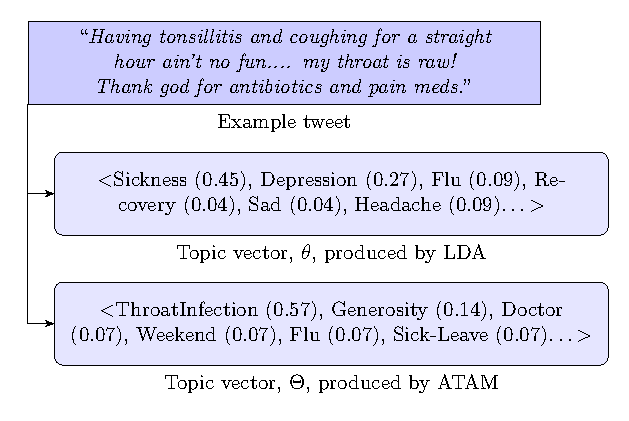
\includegraphics[width=0.45\textwidth]{tikz/exampleTweet3.pdf}
\caption{\lda vs \atam: Comparison of topic distributions for an example tweet.}
\label{fig:ldavsatam}
\end{figure}
\subsection{Ailment prediction problem}
\begin{figure}[b!]
\centering
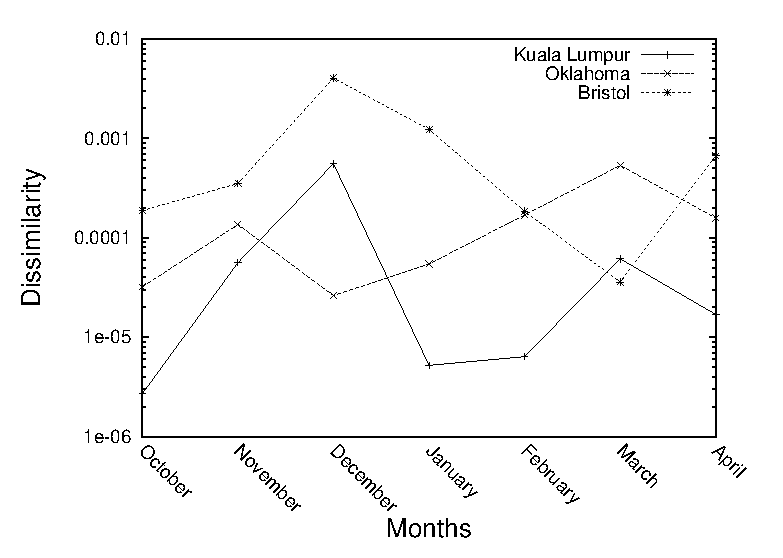
\includegraphics[width=0.45\textwidth]{gnuplot/distributiondifference/bhattacharyadistance.eps}
\caption{Topic transitions over time.}
\label{fig:ailmentsEvolve}
\end{figure}
In ~\cite{DBLP:conf/kdd/WangAB12}, \tmlda was introduced to extend \lda with modeling topic evolution over time. However, While being quite elegant in modeling general-purpose topics \tmlda is
not specialized to capture \texttt{\emph{health}} transitions over time.

Let $\Theta_g^t$ be a ailment distribution vector where the weight of each ailment is representative of the discourse density of ailment in the tweets originating from region $g$ during period $t$.
For a region $g$, the interval of time spanning a set of consecutive time periods $\{t_i,t_{i+1},\ldots\}$ during which discovered ailment distributions  $\{\Theta_g^{t_i},\Theta_g^{t_{i+1}},\ldots\}$
do not change appreciably forms a \season w.r.t. ailments. By definition, a \season is (nearly) homogeneous in terms
of ailments. In other words, the ailments evolve in a smooth fashion
within a \season and change abruptly across \season boundary. We posit that such \seasons exist after which they encounter \changes in ailment topic discussions. These \changes in ailment topic discussions 
may be caused by onset of the disease or some other external factors. Nevertheless, they are the interesting points for analyzing purposes.
As an example, in Figure~\ref{fig:ailmentsEvolve}, we show the difference between ailment distributions of consecutive months for 3 different regions Kuala Lumpur (a city in Indonesia), Oklahoma (a state in the USA), and Bristol (a city in the UK). The sharp peaks obtained validate the existence of time intervals that are homogeneous w.r.t. ailments.
\begin{algorithm}[t!]
\caption{TM-ATAM: \change Detection and Training Ailment Distribution Predictor}
\label{alg:tmatam}
\begin{algorithmic}[1]
 \ForAll {$g \in G$}\label{alg:line:start}
 \State Run ATAM on $D_g$\label{alg:line:atam}
 \ForAll  {$t \in \mf T$}:\label{alg:line:tstart}
 \ForAll {$z \in \mf Z$}:\label{alg:line:createThetaStart}
 \State $\Theta_g^t[z] \leftarrow 0$
 \EndFor
 \ForAll {$d \in D_g^t$}:
 \ForAll {$w \in d$}:
 \State $z \gets topic(w)$
 \State $\Theta_g^t[z] \gets \Theta_g^t[z] + \frac{1}{|d|\times |D_g^t|}$
 \EndFor
 \EndFor\label{alg:line:createThetaEnd}
 \EndFor
 \State $\displaystyle t_{c} = \argmax_t{\ m(\Theta_g^{t-1},\ \Theta_g^{t})}$\label{alg:line:ThetaDiff}
 \State $pre = [t_1\ ,\ t_{c-1}]$\label{alg:line:buildSeasonPre} 
 \State $post = [t_{c}\ , \ t_{|\mf T|}]$\label{alg:line:buildSeasonPost} 
 \ForAll {$s \in \{pre,\ post\}$}:\label{alg:line:predStart}
 \State $A_g^t\approx A_g^{t-1}.M$
 \State $M =(A_g^{t-1\intercal}A_g^{t-1})^{-1}A_g^{t-1\intercal}A_g^t$
 %\State $M = A_g^{t-1}\textsuperscript{\textdagger}A_g^t=(A_g^{t-1\intercal}A_g^{t-1})^{-1}A_g^{t-1\intercal}A_g^t$
 \EndFor\label{alg:line:predEnd}
\EndFor\label{alg:line:end}
\end{algorithmic}
\end{algorithm}

\label{subsec:problem}
{\bf Our problem:} Given a set of
documents $D_g^{t_{i-1}}$ formed by tweets originating from a region
$g \in G$ during time period $t_{i-1}$, predict $\Theta_g^{t_i}$, the
ailment distribution of documents in $D_g^{t_i}$, corresponding to
posts from $g$ in period $t_i$ from $\Theta_g^{t_{i-1}}$, the ailment
distribution of document $D_g^{t_{i-1}}$ corresponding to posts from
$g$ during period $t_{i-1}$.
\subsection{Modeling Health Topics over Time with \tmatam}
\label{subsec:model}
To solve our problem, we propose \tmatam that builds on top of \atam and \tmlda.
We first convert inferences of \atam over a single document to associate with a given set of documents $D_g^t$, an ailment
distribution, $\Theta_g^t$. We then go on to find \seasons. We model ailment transitions within each \season and when a \change is 
encountered we update these transitions.  This is a fresh departure
from existing solutions that operate in a \season-agnostic fashion\cite{DBLP:conf/kdd/WangAB12}.
\tmatam, at its heart, solves the following equation.
\begin{equation}
A_g^{t}\approx A_g^{t-1}.M^*
\end{equation}
where
\begin{equation}
A_g^{t-1}=\begin{pmatrix}\Theta_g^1\\\vdots\\\Theta_g^t\end{pmatrix},\,A_g^t=\begin{pmatrix}\Theta_g^2\\\vdots\\\Theta_g^{t+1}\end{pmatrix}
\end{equation}
$M^*$ is an unknown transition matrix which is obtained by solving the following least squares problem.
\[
M^*=\mathop{argmin}_M\|A_g^t- A_g^{t-1}.M\|_F
\]
Algorithm~\ref{alg:tmatam} contains the steps of our solution. It has 
two parts:  \change \emph{\texttt{detection}} and \emph{\texttt{ailment prediction}}. 
\paragraph{Change Point Detection}
We use $\mf Z$ to refer to the set of all health-related and
non-health related topics. For each region $g \in \mf G$
(Line~\ref{alg:line:start}) we first run \atam over the full time
period $D_g$ (Line~\ref{alg:line:atam}).  Next for each period $t\in
\mf T$ (Line~\ref{alg:line:tstart}), we use the output of \atam over
$D_g$ to generate a topic distribution $\Theta_g^t$
(Lines~\ref{alg:line:createThetaStart}--
\ref{alg:line:createThetaEnd}).  We then examine the
\emph{Bhattacharyya Distance} between consecutive distributions
$\Theta_g^{t-1}$ and $\Theta_g^t$ of the region $g$ to identify the
most significant \change, $t_c$, for region $g$ (Line~\ref{alg:line:ThetaDiff}). The
time periods preceding and succeding \change are termed as \seasons.
\paragraph{Ailment Prediction}
In the second module of \tmatam algorithm, we predict distribution of ailments in twitter discourse ahead of time for each \season.
Lines~\ref{alg:line:predStart}--\ref{alg:line:predEnd} 
of Algorithm~\ref{alg:tmatam} outline the steps undertaken to identify the detection of ailments for intra-homogeneous periods.

\section{Experiments}
\label{sec:results}
We conducted experiments to evaluate the performance of \tmatam  and to compare with the state of the art. 
\subsection{Experimental setup}
\label{subsec:setup}
%\subsubsection{Data}
We employ Twitter's Streaming API to collect tweets between $2014$-Oct-$8$ and $2015$-May-$31$. Collected tweets were subjected to two pre-processing steps as follows.


{\bf Identifying health-related tweets:} We filter the tweets 
returned by the \emph{Decahose Stream} to obtain \emph{health-related} 
tweets. We say that a tweet is health-related if it contains a health 
keyword and passes our classification criteria.  We used 20,000 health-related keywords crawled from
wrongdiagnosis.com to first filter the tweets.
The process is then automated with the help of an SVM classifier~\cite{DBLP:journals/ml/CortesV95}. To this end, $5128$ tweets were 
 annotated through crowdsourcing efforts. The precision and recall of the 
 classifier are $0.85$ and $0.44$. Table~\ref{tab:data:stats} 
shows that out of the 1.36B tweets we collected, 698K were health-related.
\begin{table}[t!]
\centering
\caption{Dataset Statistics}
\label{tab:data:stats}
{\small \begin{tabular}{|c|c|}
\hline
collection period (days) & 235\\
\hline
\#tweets & {1,360,705,803}\\
\hline
\#tweets (health-related) & 698,212\\
\hline
\#tweets (health-related+geolocated) & 569,408\\
\hline
\end{tabular}
}
\end{table}

{\bf Identifying geolocalized tweets:} The ability to operate
seamlessly at varying geographic resolutions mandates that the exact
location of each tweet be known to \tmatam. Twitter affords its users
the option to share their geolocation. In our
case, over half a million tweets are retained ($569K$ as indicated in
Table~\ref{tab:data:stats}).

We examine various choices for the geographic granularities, temporal
granularities and distance measures. \tmatam performs better on
smaller regions. We attribute this
result to the fact that tweets from smaller regions show less diversity in topics. We also found weekly ailment distributions to be very sparse. We also used 2 distance measures to measure distribution difference
namely, cosine similarity and Bhattacharyya distance. We observed that
number of tweets at a given time granularity $t$ may affect the
performance of Cosine Similarity. Finally, we chose to work with geographic granularity of \texttt{\emph{states}}, temporal granularity of \texttt{\emph{months}} and distance measure of \texttt{\emph{Bhattacharyya}}.

{\bf Test-bench and measures:} We run our experiments on a {32 core Intel Xeon @ 2.6Ghz CPU 
(with 20MB cache per core)} system with {128 Gig} RAM running 
{Debian GNU/Linux 7.9 (wheezy)} operating system.
All subsequently discussed components were implemented in 
Java {1.8.0\_60}. 
We used \emph{perplexity} to compare between models \cite{Wallach:2009:EMT:1553374.1553515}.
\subsection{Experimental Results}
Recall that the terms \change and \season refer to the point in time at which discourse density of ailments changes substantially, and the time period before and after that point, respectively. We  divide each \season into training and test sets. \atam is then \emph{\texttt{re-run}} over the training set of each \season. We then model a \transition  \emph{\texttt{$M_{tmatam}^*$}} on the training set of each \season as described in Section~\ref{subsec:model}. We compute the probability of "health topic" $z$ for each tweet $p$ of the first month ($|\mf T|-1$) in the test set using the following formulas:
\begin{equation}
\label{eq:probabilitytopicgiventimepost}
P(z|t_{|\mf T|-1}) = \frac{\sum_{p\ \in t_{|\mf T|-1}}P(z|p\ for\ t_{|\mf T|-1} )}
    {\# tweets\ for\ t_{|\mf T|-1}}
\end{equation}
\begin{equation}
P(z|p)=\sum_{w}P(z|w)P(w|p) = \sum_{w}\frac{n(z,w)}{n(w)}P(w|p)
\end{equation}
Here, values for $n(z,w)$,$n(w)$ are taken from \atam run on the training months. P(w|p) is simply the number of times word $w$ occurs in the tweet $p$ divided by the total number of words in $p$.
We then predict the future probability of each topic in the second month of the test data using the corresponding \transition $M_{tmatam}^*$. Probability of word $p_l(w_i)$ for any document set is calculated as follows:
\begin{equation}
\label{eq:probabilityword}
p_l(w_i)=\sum_{z}P(w|z)P(z) = \sum_{z}\frac{n(z,w)}{n(z)}P(z)
\end{equation}
Having computed $P(w)$, we can compute perplexity against the words of the tweets of second test month.
\subsubsection{\tmatam vs \atam, \tmlda vs \lda}
Figure \ref{fig:perplexity} shows the perplexity ratio of \tmatam with state-of-the art models. If ratio computes to be less than "1" for \competitor, \tmatam is performing worse. If ratio is more than "1" for \competitor, \tmatam is performing better. In order to assert the fact that health topics transit from one to another, we compute the perplexity of \atam on words of the \textit{first month} of the test set and not predicting any topic distribution using any \transition. Hence, this denotes the case where health topics stay \texttt{\emph{static}}. As shown in Figure~\ref{fig:perplexity}, \tmatam beats \atam in all social media active regions (an active region is a region where the proportion of tweets if high enough). For training {\tmlda}, we merge the training data (same as \tmatam) of each \season in each region and train a \transition of \tmlda by solving least squares problem. For each tweet $p$ of the first month of the test set, we compute the probability of topics using LDA trained on merged training data (Formula \ref{eq:probabilitytopicgiventimepost}). We then predict the future probability of each topic in the following month using  $M_{tmlda}^*$. We can then compute the perplexity of \tmlda against words of actual tweets in the test set. Figure~\ref{fig:perplexity} shows that \tmatam consistently beats \tmlda and \lda in predicting future health topics on the test month. Perplexity is indeed lower for all words of the test month in all active states.
\begin{figure}[t!]
\centering
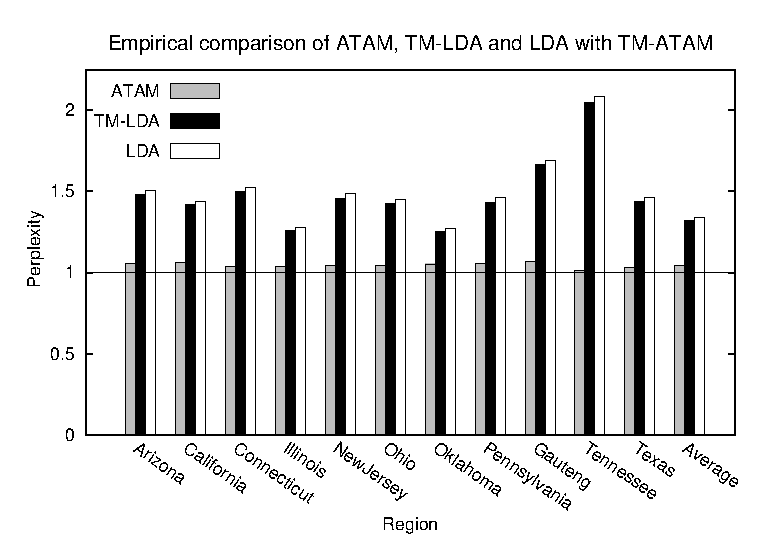
\epsfig{file=gnuplot/perplexity/perplexityRatio2,width=0.45\textwidth}
\caption{Comparison for top 10 active regions. Histograms denote ratio of perplexities. \tmatam is always at 1.0.}  %If ratio is less than "1" for \competitor, \tmatam is performing worse. If ratio is more than "1" for \competitor, \tmatam is performing better.}
\label{fig:perplexity}
\end{figure}
\subsubsection{Homogenous Time Periods}
\label{subsubsec:season}
In Figure \ref{fig:seasonBoundary:NonUS}
we show the top-2 sharpest \changes for the top regions. Those points can be explained with weather
changes in those regions. Texas can be explained with a
drop in temperature while Jervis Bay can be explained by an increase in
rainfall. Dublin sees its lowest temperature in November.
Singapore and Manila have very similar weather conditions and exhibit
the same change point.
\begin{figure}[h!]
\centering
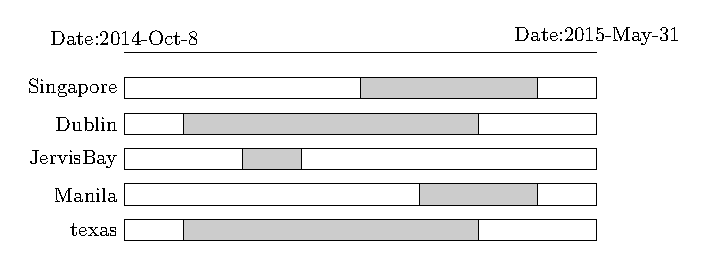
\includegraphics[width=0.45\textwidth]{tikz/seasons_short.pdf}
\caption{Top-2 Monthly \season for top active regions.}
\label{fig:seasonBoundary:NonUS}
\end{figure}
\subsubsection{Topic Transitions}
Entry $m_{ij}$ in the \transition $M$ produced by
\tmatam, shows the degree that topic $z_i$ will contribute to topic $z_j$
in the subsequent \season.
We adapt the threshold used in \cite{DBLP:conf/kdd/WangAB12} to our settings: Threshold  = $\mu + 2\times\sigma_{non-diagonal}$.
We identify two kinds of interesting transitions based on the above threshold:
 \texttt{\emph{selftransitions}}: popular topics and \texttt{\emph{one way transitions}}: $i^{th}$ topic is discussed before $j^{th}$ topic.
As an example, one-way-transitions of California are summarized in Table \ref{tab:fulltransitionCalifornia}.
\begin{table}[t!]
\centering
\caption{One-Way Transitions for California (threshold: $0.815$)}
\label{tab:fulltransitionCalifornia}
{\small \begin{tabular}{|c|c|l|} \hline
 From Topic&To Topic&Weight\\ \hline
  smoking/junkies & respiratory diseases&  2.70\\ /drugs/cigarettes & & \\ \hline
  depression/complaining &  joint pains/body pains&  3.25\\ /cursing/slangs/self-pity & & \\
 \hline\end{tabular} 
}
\end{table}

\section{Conclusion}
\label{sec:conclusion}
We studied how to uncover ailment distributions over time in social
media.  We proposed a granularity-based model to conduct
region-specific analysis that leads to the identification of time
intervals characterizing homogeneous ailment discourse, per region.
We modeled disease evolution within each homogeneous
region and attempted to predict ailments.  The fine-grained nature of
our model results in significant improvements over state of the art
methods.  %% We envisage a use case where our ailment predictions can
%% replace existing solutions for syndromic surveillance that
%% are both costly and time consuming.


%\section{The {\secit Body} of The Paper}
%\subsection{Type Changes and {\subsecit Special} Characters}

% Proforma: table (normal)
%    \begin{table}
%        \centering
%        \caption{Frequency of Special Characters}
%        \begin{tabular}{|c|c|l|} \hline
%            Non-English or Math&Frequency&Comments\\ \hline
%            \O & 1 in 1,000& For Swedish names\\ \hline
%            $\pi$ & 1 in 5& Common in math\\ \hline
%            \$ & 4 in 5 & Used in business\\ \hline
%            $\Psi^2_1$ & 1 in 40,000& Unexplained usage\\
%        \hline\end{tabular}
%    \end{table}

%% Proforma: table (wide)
%    \begin{table*}
%        \centering
%        \caption{Some Typical Commands}
%        \begin{tabular}{|c|c|l|} \hline
%            Command&A Number&Comments\\ \hline
%            \texttt{{\char'134}alignauthor} & 100& Author alignment\\ \hline
%            \texttt{{\char'134}numberofauthors}& 200& Author enumeration\\ \hline
%            \texttt{{\char'134}table}& 300 & For tables\\ \hline
%        \texttt{{\char'134}table*}& 400& For wider tables\\ \hline\end{tabular}
%        \end{table*}

% Proforma: Math (inline)
%    \begin{math}\lim_{n\rightarrow \infty}x=0\end{math}

    % Proforma: Math (numbered)
%    \begin{equation}\lim_{n\rightarrow \infty}x=0\end{equation}

    % Proforma: Math (non numbered)
%    \begin{equation}\lim_{n\rightarrow \infty}x=0\end{equation}

% Proforma: theorem 
%\newtheorem{theorem}{Theorem}
%\begin{theorem}
%    Let $f$ be continuous on $[a,b]$.  If $G$ is
%    an antiderivative for $f$ on $[a,b]$, then
%\begin{displaymath}\int^b_af(t)dt = G(b) - G(a).\end{displaymath}
%\end{theorem}
%

%Proforma: definition
%\newdef{definition}{Definition}
%\begin{definition}
%    If $z$ is irrational, then by $e^z$ we mean the
%    unique number which has
%logarithm $z$: \begin{displaymath}{\log e^z = z}\end{displaymath}
%\end{definition}


% Proforma: proof
%\begin{proof}
%    Suppose on the contrary there exists a real number $L$ such that
%    \begin{displaymath}
%        \lim_{x\rightarrow\infty} \frac{f(x)}{g(x)} = L.
%    \end{displaymath}
%    Then
%    \begin{displaymath}
%        l=\lim_{x\rightarrow c} f(x)
%        = \lim_{x\rightarrow c}
%        \left[ g{x} \cdot \frac{f(x)}{g(x)} \right ]
%        = \lim_{x\rightarrow c} g(x) \cdot \lim_{x\rightarrow c}
%        \frac{f(x)}{g(x)} = 0\cdot L = 0,
%    \end{displaymath}
%    which contradicts our assumption that $l\neq 0$.
%\end{proof}

\bibliographystyle{abbrv}
\bibliography{./bib/references_short} 
%\balancecolumns
\end{document}
